% !TeX program = xelatex
% Сводный конспект лекций 1--3 по теории пучков, курс С. М. Львовского.
% Лекция 2 включена из готового lecture-02/lecture-2.pdf.
\documentclass[11pt,b5paper,oneside]{article}

\usepackage{fontspec}
\usepackage{polyglossia}
\setdefaultlanguage{russian}
\setotherlanguage{english}
\defaultfontfeatures{Ligatures=TeX}
\setmainfont{PT Serif}

\usepackage{geometry}
\geometry{b5paper,inner=1.65cm,outer=1.35cm,top=1.55cm,bottom=1.3cm,
  headsep=7pt}
\usepackage{amsmath,amssymb,amsthm,mathtools,mathrsfs}
\usepackage{tikz}
\usetikzlibrary{arrows.meta,positioning,calc}
\usepackage{tikz-cd}
\usepackage{booktabs,array,enumitem,titlesec,titletoc,fancyhdr,needspace}
\usepackage[final]{microtype}
\usepackage[unicode,linktocpage=true,colorlinks=true,
  linkcolor=black,citecolor=black,urlcolor=blue]{hyperref}
\usepackage{pdfpages}

\definecolor{ink}{HTML}{17202A}
\definecolor{accent}{HTML}{A63D40}
\AtBeginDocument{\color{ink}}
\setlength{\emergencystretch}{3em}
\setlist{nosep,leftmargin=*}
\setlist[enumerate,1]{label=(\arabic*),leftmargin=*}
\setlist[itemize,1]{label=--,leftmargin=1.2em}
\pagestyle{fancy}
\fancyhf{}
\renewcommand{\headrulewidth}{0.4pt}
\fancyhead[L]{\footnotesize Теория пучков: лекции 1--3}
\fancyhead[R]{\footnotesize\thepage}
\titleformat{\section}[block]{\normalfont\Large\bfseries}{\thesection.}{.5em}{}
\titlespacing*{\section}{0pt}{17pt}{8pt}
\titleformat{\subsection}[runin]{\normalfont\bfseries}{\thesubsection.}{.5em}{}[.]
\titlespacing{\subsection}{0pt}{1.4ex}{.8em}

\newcommand{\F}{\mathscr F}
\newcommand{\G}{\mathscr G}
\newcommand{\I}{\mathscr I}
\newcommand{\Hh}{\mathscr H}
\newcommand{\Sh}{\mathrm{Sh}}
\newcommand{\PSh}{\mathrm{PSh}}
\newcommand{\Ab}{\mathrm{Ab}}
\newcommand{\id}{\mathrm{id}}
\newcommand{\res}{\rho}
\newcommand{\et}{\mathrm{\acute Et}}
\newcommand{\im}{\operatorname{im}}
\newcommand{\coker}{\operatorname{coker}}
\newcommand{\Hom}{\operatorname{Hom}}
\newcommand{\Spec}{\operatorname{Spec}}
\newcommand{\Gammafun}{\Gamma}
\newcommand{\R}{\mathbb R}
\newcommand{\C}{\mathbb C}
\newcommand{\Z}{\mathbb Z}

\theoremstyle{plain}
\newtheorem{thm}{Теорема}[section]
\newtheorem{lem}[thm]{Лемма}
\newtheorem{cor}[thm]{Следствие}
\theoremstyle{definition}
\newtheorem{defn}[thm]{Определение}
\newtheorem{exm}[thm]{Пример}
\theoremstyle{remark}
\newtheorem{rem}[thm]{Замечание}

\newcommand{\source}[1]{\par\smallskip{\footnotesize\itshape Источники и параллели: #1}\par\smallskip}
\newcommand{\diagstyle}{column sep=large,row sep=large,every node/.style={font=\small}}

\begin{document}

\thispagestyle{empty}
\vspace*{1.3cm}
\begin{center}
{\Large Конспект лекций 1--3\par}
\vspace{.7cm}
{\LARGE\bfseries Предпучки, пучки и локально-глобальные\par}
{\LARGE\bfseries методы в теории пучков\par}
\vspace{.8cm}
{\large Курс С.~М.~Львовского\par}
\vspace{1.2cm}
\begin{minipage}{.82\textwidth}
\centering
Конспект собран по рукописным сканам лекций 1--3 и готовому
конспекту лекции~2. Изложение дополнено мотивациями и развернутыми
доказательствами. В местах, где нестрогое бытовое описание могло бы
смешать разные понятия, явно указаны точные определения: в частности,
различаются предпучковый и пучковый образ, точность пучков и точность
глобальных сечений.
\end{minipage}
\vfill
{\small Формат B5\par}
\end{center}
\clearpage

\tableofcontents
\clearpage

%==================================================================
\section{Как устроен курс: локальные данные и глобальные объекты}
%==================================================================

\subsection{Главный вопрос}
Теория пучков систематизирует переход от объектов, определённых
локально, к объектам на всём пространстве. Во всех примерах ниже
возникают две разные задачи:
\begin{itemize}
\item существуют ли локальные решения в окрестности каждой точки;
\item можно ли эти локальные решения согласовать и склеить в глобальное.
\end{itemize}
Вторая задача не сводится к первой: препятствие может быть топологическим.
Пучок хранит не только множество локальных объектов, но и точные правила
их ограничения и склейки.

\begin{exm}[локальный логарифм]
Пусть $U\subset\C$ открыто и $f:U\to\C^\times$ голоморфна.
В каждой точке $a\in U$ можно выбрать достаточно малую окрестность $V$
и голоморфную функцию $g$ на $V$ такую, что $e^g=f|_V$. Глобальный
логарифм, однако, может не существовать. Для $U=\C^\times$ и $f(z)=z$
его отсутствие следует, например, из
\[
  \int_{|z|=1}\frac{f'(z)}{f(z)}\,dz=2\pi i,
\]
тогда как при $f=e^g$ интеграл равнялся бы $\int_{|z|=1}dg=0$.
\end{exm}

\begin{exm}[замкнутая, но не точная форма]
На ориентированной сфере $S^2$ форма площади $\omega$ замкнута, поскольку
$d\omega=0$ по размерности. Она не точна: если $\omega=d\eta$, то по
теореме Стокса
\[
  \int_{S^2}\omega=\int_{S^2}d\eta=\int_{\partial S^2}\eta=0,
\]
но интеграл формы площади положителен. На достаточно малых координатных
окрестностях замкнутая форма точна по лемме Пуанкаре. И здесь локальная
разрешимость не влечёт глобальную.
\end{exm}

Обе ситуации подсказывают одну и ту же конструкцию: сопоставлять каждому
открытому множеству группу локальных решений и при включении открытых
множеств ограничивать решение. Это и есть исходные данные предпучка.

\subsection{Дорожная карта}
Первая лекция вводит предпучки, пучки, ростки и ассоциированный пучок.
Вторая строит ассоциированный пучок через пространство ростков и
доказывает его универсальное свойство. Третья рассматривает глобальные
сечения, их точность, фласковые пучки и переход к когомологиям.

%==================================================================
\section{Предпучки, морфизмы и пучки}
%==================================================================

\subsection{Предпучок как контравариантный функтор}
Пусть $X$ --- топологическое пространство, а $\operatorname{Open}(X)$ ---
категория его открытых подмножеств, где морфизмы --- включения.

\begin{defn}[предпучок абелевых групп]
Предпучок $\F$ на $X$ задаёт абелеву группу $\F(U)$ каждому открытому
$U\subset X$ и гомоморфизм ограничения
\[
  \res^V_U:\F(V)\longrightarrow\F(U),\qquad U\subset V,
\]
причём
\[
  \res^U_U=\id,\qquad
  \res^W_U\circ\res^V_W=\res^V_U
  \quad(U\subset W\subset V).
\]
Эквивалентно, это контравариантный функтор
$\F:\operatorname{Open}(X)^{\mathrm{op}}\to\Ab$.
\end{defn}

Для $s\in\F(V)$ пишут $s|_U=\res^V_U(s)$. Слово «сечение» здесь
обозначает элемент $\F(U)$; это не обязательно функция на $U$.
Функториальность кодирует согласованность всех последовательных
ограничений.

\begin{exm}[функции и формы]
Назначения $U\mapsto C(U,\R)$, $U\mapsto C^\infty(U)$,
$U\mapsto\Omega^k(U)$ с обычными ограничениями являются предпучками.
Внешняя производная совместима с ограничениями, поэтому задаёт морфизм
предпучков $d:\Omega^k\to\Omega^{k+1}$.
\end{exm}

\begin{defn}[морфизм предпучков]
Морфизм $f:\F\to\G$ --- семейство гомоморфизмов
$f_U:\F(U)\to\G(U)$, коммутирующих с ограничениями:
\[
  f_U(s|_U)=f_V(s)|_U\qquad(U\subset V,\ s\in\F(V)).
\]
То есть морфизм предпучков есть естественное преобразование функторов.
\end{defn}

Ядро и образ можно сначала определить поточечно в категории предпучков:
\[
 (\ker f)(U)=\ker(f_U),\qquad
 (\operatorname{im}_{\mathrm{pre}} f)(U)=\operatorname{im}(f_U).
\]
Оба назначения являются предпучками. Но поточечный образ не обязан
удовлетворять аксиоме склейки и потому в общем случае не является
пучком. Это различие будет существенно ниже.

\subsection{Аксиомы пучка}
\begin{defn}[пучок]
Предпучок $\F$ называется пучком, если для любого открытого $U$ и любого
открытого покрытия $U=\bigcup_{i\in I}U_i$ выполнены условия:
\begin{enumerate}
\item[(F0)] $\F(\varnothing)=0$;
\item[(F1)] если $s,t\in\F(U)$ и $s|_{U_i}=t|_{U_i}$ для всех $i$, то
  $s=t$;
\item[(F2)] если $s_i\in\F(U_i)$ и
  $s_i|_{U_i\cap U_j}=s_j|_{U_i\cap U_j}$ для всех $i,j$, то существует
  единственное $s\in\F(U)$ с $s|_{U_i}=s_i$.
\end{enumerate}
\end{defn}

Условие согласованности в (F2) включает пустые пересечения: оно там
автоматически выполнено, так как $\F(\varnothing)=0$. (F1) говорит, что
данные определяются локально; (F2) --- что совместимые локальные данные
действительно происходят из глобального сечения. Единственность в (F2)
следует из (F1), но её удобно включать в формулировку.

Для пучка абелевых групп и фиксированного покрытия условие можно записать
как точность начала последовательности
\[
  0\longrightarrow\F(U)\longrightarrow
  \prod_i\F(U_i)\mathrel{\substack{\longrightarrow\\[-.6ex]\longrightarrow}}
  \prod_{i,j}\F(U_i\cap U_j),
\]
где первое отображение состоит из ограничений, а равенство двух
последующих компонент означает согласованность. Важно: требуется
точность в первых двух ненулевых местах, но не сюръективность последнего
отображения.

\subsection{Базовые примеры и контрпримеры}
\begin{exm}[постоянный предпучок и постоянный пучок]
Постоянный предпучок со значением $A$ задаётся равенством
$\F(U)=A$ для непустых $U$ и $\F(\varnothing)=0$, а все ограничения
между непустыми открытыми --- тождественные. Если $U$ несвязно, локальные
значения $a_1,a_2\in A$ на двух непересекающихся открытых кусках не обязаны
совпадать, поэтому не могут склеиться в один элемент $A$. Значит,
постоянный предпучок в общем случае не пучок.

Ассоциированный ему постоянный пучок $\underline A$ задаётся формулой
\[
  \underline A(U)=\{\text{локально постоянные отображения }U\to A\},
\]
где $A$ снабжено дискретной топологией. При связном $U$ такие отображения
постоянны; при несвязном они могут принимать различные значения на
разных компонентах.
\end{exm}

\begin{exm}[ограниченные функции не образуют пучок]
Пусть $X=\R$ и $\F(U)$ --- группа ограниченных непрерывных функций на
$U$. Функция $f(x)=x$ ограничена на каждом $U_n=(-n,n)$, а семейство
$f|_{U_n}$ согласовано и покрывает $\R$. Его склейка в пучке непрерывных
функций есть $f$, но $f\notin\F(\R)$. Следовательно, аксиома (F2)
нарушается.
\end{exm}

\begin{exm}[замкнутые и точные формы]
Назначение $U\mapsto Z^k(U)=\ker(d:\Omega^k(U)\to\Omega^{k+1}(U))$
является пучком: условие $d\omega=0$ проверяется локально, а формы
склеиваются как сечения пучка $\Omega^k$.

Напротив, $B^k(U)=d\Omega^{k-1}(U)$ --- поточечный образ $d$ и обычно
лишь предпучок. Например, на $S^1$ глобальная форма угла $d\theta$ имеет
локальные первообразные на дугах, но не является дифференциалом глобальной
функции: её интеграл по окружности ненулевой. Поэтому локально точные
формы склеиваются как формы, но полученная форма может не быть глобально
точной. Ассоциированный пучок к $B^k$ описывает формы, локально точные;
для $k\geq1$ по лемме Пуанкаре это пучок замкнутых форм на гладком
многообразии.
\end{exm}

\subsection{Ядро пучкового морфизма}
\begin{thm}
Если $f:\F\to\G$ --- морфизм пучков абелевых групп, то поточечное ядро
$\ker f$ является пучком.
\end{thm}
\begin{proof}
Условие (F0) выполняется для ядра нулевое. Для (F1) достаточно применить
(F1) в $\F$. Для (F2) пусть $s_i\in\ker(f_{U_i})$ согласованы. Сначала
их склеиваем в $s\in\F(U)$ по (F2) для $\F$. На каждом $U_i$
ограничение $f_U(s)$ равно $f_{U_i}(s_i)=0$. По (F1) для $\G$ имеем
$f_U(s)=0$, так что $s\in\ker(f_U)$. Единственность также следует из
(F1) для $\F$.
\end{proof}

\begin{rem}[почему с образом иначе]
Образ морфизма в категории пучков --- это не обязательно предпучок
$U\mapsto\operatorname{im}(f_U)$, а его ассоциированный пучок. Элемент
пучкового образа локально, но не обязательно глобально, представим как
$f(s)$. Для форм это ровно различие между глобально точными и локально
точными формами. Подмена пучкового образа поточечным образом приводит к
ложным утверждениям о точности.
\end{rem}

\source{Для формулировок о пучках и представлении пучка через étale-пространство см. Mac Lane--Moerdijk, часть II, §§1--7; Tennison, гл. 1--3; Iversen, гл. 2.}

%==================================================================
\section{Лекция 2: пространство ростков и ассоциированный пучок}
%==================================================================

Вторая лекция включена целиком по готовому конспекту, подготовленному по
сканам страниц 9--15 тетради. Сохраняются исходная последовательность
изложения, доказательства, диаграммы и дополнения по Годеману и Манину.
\par\medskip
\noindent\textbf{Главные результаты раздела:} ростки как прямые пределы;
étale-пространство $\et(\F)$; пучок непрерывных сечений
$\F^\sharp$; универсальное свойство
\[
  \Hom_{\PSh(X)}(\F,\G)\simeq
  \Hom_{\Sh(X)}(\F^\sharp,\G)
  \quad(\G\in\Sh(X));
\]
совпадение построений $\F^+$ и $\F^\sharp$; критерий точности через
слои.

\clearpage
\phantomsection
\addcontentsline{toc}{subsection}{Полный текст конспекта лекции 2 (страницы 9--15 тетради)}
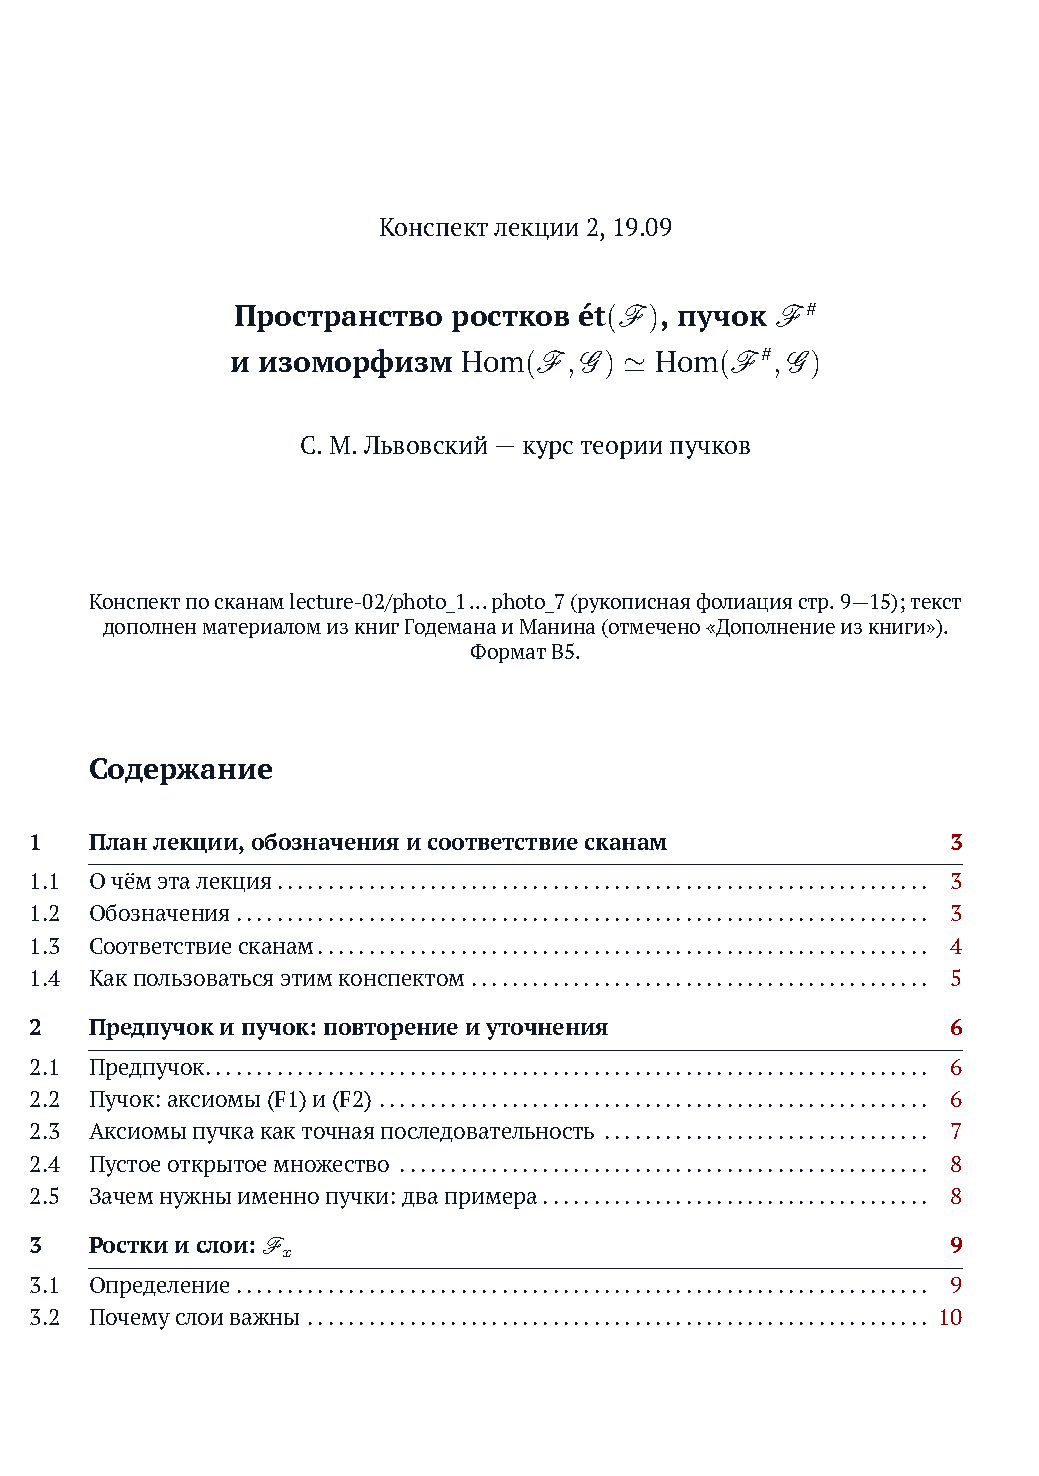
\includepdf[pages=-,pagecommand={\thispagestyle{empty}}]{lecture-02/lecture-2.pdf}
\clearpage

%==================================================================
\section{Лекция 3: глобальные сечения и когомологии}
%==================================================================

\subsection{Функтор глобальных сечений}
Пусть $\F$ --- пучок на $X$. Его группа глобальных сечений обозначается
\[
  \Gamma(X,\F)=\F(X).
\]
Морфизм $f:\F\to\G$ индуцирует гомоморфизм
$\Gamma(X,f):\F(X)\to\G(X)$. Таким образом, $\Gamma(X,-)$ --- ковариантный
функтор $\Sh(X)\to\Ab$.

\begin{thm}[глобальные сечения сохраняют левую часть точности]
Если
\[
  0\longrightarrow\F\xrightarrow{i}\G\xrightarrow{q}\Hh
\]
точна как последовательность пучков, то
\[
  0\longrightarrow\F(X)\xrightarrow{i_X}\G(X)
  \xrightarrow{q_X}\Hh(X)
\]
точна как последовательность абелевых групп.
\end{thm}
\begin{proof}
Для пучков точность равносильна точности последовательности ростков
в каждой точке. Если $i_X(s)=0$, то $i_x(s_x)=0$ для всякого $x$;
инъективность $i_x$ даёт $s_x=0$. Пучковая аксиома единственности
влечёт $s=0$, значит $i_X$ инъективно.

Теперь пусть $t\in\G(X)$ и $q_X(t)=0$. Для каждого $x\in X$ точность
на ростке даёт $t_x\in\ker q_x=\operatorname{im}i_x$. По определению
ростка это означает, что в некоторой окрестности $U_x$ существует
$s_x\in\F(U_x)$ с $i(s_x)=t|_{U_x}$. На пересечении $U_x\cap U_y$
имеем $i(s_x|)=t|=i(s_y|)$; инъективность морфизма пучков $i$ даёт
$s_x|=s_y|$. По аксиоме склейки они склеиваются в $s\in\F(X)$,
причём $i_X(s)=t$. Обратное включение $\operatorname{im}i_X\subseteq
\ker q_X$ следует из $q\circ i=0$.
\end{proof}

Это утверждение не говорит, что $\F(X)\to\G(X)\to\Hh(X)$ сюръективно
на $\Hh(X)$. Эпиморфизм пучков означает локальную сюръективность на
сечениях, а не обязательное наличие глобального подъёма.

\begin{exm}[экспоненциальная последовательность]
На комплексном гладком многообразии имеется короткая точная
последовательность пучков абелевых групп
\[
  0\longrightarrow\underline{\Z}
  \longrightarrow\mathcal C^\infty_{\C}
  \xrightarrow{\ z\mapsto e^{2\pi iz}\ }
  \mathcal C^\infty_{\C^\times}\longrightarrow 1.
\]
Точность справа локальна: всякая гладкая функция со значениями в
$\C^\times$ имеет локальный гладкий логарифм. На $S^1$ глобальная функция
$z\mapsto z$ не имеет глобального логарифма, поэтому отображение глобальных
сечений справа не сюръективно. Препятствие измеряет ненулевое число
наматывания.
\end{exm}

\subsection{Точность проверяется на ростках}
Для морфизма пучков $f:\F\to\G$ индуцируются морфизмы ростков
$f_x:\F_x\to\G_x$. Прямой предел по окрестностям точен в категории
абелевых групп, поэтому
\[
  (\ker f)_x\simeq\ker(f_x),\qquad
  (\operatorname{im}_{\Sh} f)_x\simeq\operatorname{im}(f_x),\qquad
  (\coker f)_x\simeq\coker(f_x).
\]
Здесь $\operatorname{im}_{\Sh}f$ --- образ в категории пучков,
то есть ассоциированный пучок к предпучковому образу.

\begin{thm}[локальный критерий точности]
Пусть дана последовательность пучков, образующая комплекс, то есть
$d^n\circ d^{n-1}=0$ для всех $n$:
\[
  \cdots\longrightarrow\F^{n-1}\xrightarrow{d^{n-1}}\F^n
  \xrightarrow{d^n}\F^{n+1}\longrightarrow\cdots
\]
точна тогда и только тогда, когда для каждого $x\in X$ последовательность
ростков
\[
  \cdots\longrightarrow\F^{n-1}_x\xrightarrow{d^{n-1}_x}\F^n_x
  \xrightarrow{d^n_x}\F^{n+1}_x\longrightarrow\cdots
\]
точна.
\end{thm}
\begin{proof}
Система окрестностей задаёт фильтрованный прямой предел.
В категории абелевых групп фильтрованные прямые пределы точны.
Поэтому взятие ростка сохраняет ядра, образы и коядра. Рассмотрим пучок
\[
  \mathscr H^n=\ker(d^n)/\operatorname{im}_{\Sh}(d^{n-1}).
\]
Точность прямого предела даёт
\[
  (\mathscr H^n)_x\simeq
  \ker(d^n_x)/\operatorname{im}(d^{n-1}_x).
\]
Если все последовательности
ростков точны, то все ростки $\mathscr H^n_x$ нулевые. Пучок с нулевыми
ростками нулевой: каждый его элемент локально равен нулю, а затем
глобально равен нулю по (F1). Значит, исходная последовательность точна.
Обратное направление следует из точности функтора ростка.
\end{proof}

\begin{rem}[что именно означает точность]
Для последовательности пучков точность в $\G$ означает равенство
пучков $\ker(g)=\operatorname{im}_{\Sh}(f)$. Эквивалентная формулировка:
каждое сечение $s\in\G(U)$ с $g(s)=0$ локально на покрытии $U$ является
образом сечения из $\F$. Не требуется, чтобы оно было образом одного
сечения $\F(U)$ на всём $U$.
\end{rem}

\subsection{Зачем нужны высшие когомологии}
Функтор $\Gamma(X,-)$ точен слева, но не точен справа. Высшие
когомологии систематически измеряют препятствия к сюръективности и,
шире, препятствия к склейке.

Категория пучков абелевых групп на любом топологическом пространстве
имеет достаточно много инъективных объектов. Поэтому для пучка $\F$
можно выбрать инъективную резольвенту
\[
  0\longrightarrow\F\longrightarrow I^0\longrightarrow I^1
  \longrightarrow I^2\longrightarrow\cdots.
\]
Определение правых производных функтора глобальных сечений:
\[
  H^q(X,\F):=H^q\bigl(\Gamma(X,I^\bullet)\bigr).
\]
Результат не зависит с точностью до канонического изоморфизма от выбора
инъективной резольвенты.

Из определения следуют три структурных свойства:
\begin{enumerate}
\item $H^0(X,\F)\simeq\Gamma(X,\F)$ естественно по $\F$;
\item морфизм $f:\F\to\G$ индуцирует $H^q(X,f):H^q(X,\F)\to H^q(X,\G)$;
\item всякая короткая точная последовательность
  $0\to\F\to\G\to\Hh\to0$ задаёт длинную точную последовательность
  \[
  0\to H^0(X,\F)\to H^0(X,\G)\to H^0(X,\Hh)
  \xrightarrow{\delta}H^1(X,\F)\to H^1(X,\G)\to\cdots.
  \]
\end{enumerate}
Связующий гомоморфизм $\delta$ фиксирует препятствие: сечение
$h\in\Hh(X)$ поднимается до глобального сечения $\G(X)$ тогда и только
тогда, когда $\delta(h)=0$.

\source{Tennison, гл. 5, вводит когомологии как правые производные функторов; Iversen, гл. 1--2, развивает гомологический аппарат и когомологии пучков.}

\subsection{Фласковые пучки}
\begin{defn}[фласковый пучок]
Пучок $\F$ абелевых групп называется фласковым (англ. \emph{flabby},
также \emph{flasque}), если для любых открытых $V\subset U\subset X$
отображение ограничения
\[
  \F(U)\longrightarrow\F(V)
\]
сюръективно.
\end{defn}

Термин «фласковый» не следует путать с «плоским»: плоскость относится
к точности тензорного произведения и является другим свойством.

\begin{exm}
Пучок всех отображений $U\to A$ со значениями в абелевой группе $A$
фласковый: отображение с $V$ продолжается на $U$, например нулём вне
$V$. Пучок непрерывных функций обычно не фласковый: функция $1/x$ на
$(0,\infty)$ не продолжается непрерывно на $\R$.
\end{exm}

\begin{lem}
Инъективный пучок абелевых групп фласков.
\end{lem}
\begin{proof}
Для открытого $W\subset X$ обозначим через $j_{W!}\underline{\Z}_W$
продолжение нулём постоянного пучка $\Z$ с $W$ на $X$. При $V\subset U$
имеется мономорфизм
$j_{V!}\underline{\Z}_V\hookrightarrow j_{U!}\underline{\Z}_U$.
Для любого пучка $\I$ естественно
\[
  \Hom_X(j_{W!}\underline{\Z}_W,\I)\simeq\I(W).
\]
Если $\I$ инъективен, всякий морфизм $j_{V!}\underline{\Z}_V\to\I$
продлевается на $j_{U!}\underline{\Z}_U$. В указанном отождествлении
это означает сюръективность ограничения $\I(U)\to\I(V)$.
\end{proof}

\begin{thm}[фласковые пучки ацикличны]
Если $\F$ фласковый, то $H^q(X,\F)=0$ для всякого $q>0$.
Следовательно, если $0\to\F\to\G\to\Hh\to0$ --- короткая точная
последовательность и $\F$ фласковый, то
\[
  0\to\F(X)\to\G(X)\to\Hh(X)\to0
\]
точна.
\end{thm}
\begin{proof}
Возьмём инъективную резольвенту $\F\to I^\bullet$ и обозначим через
$K^0=\F$ и $K^{n+1}$ последовательные коядра в точных коротких
последовательностях
\[
  0\longrightarrow K^n\longrightarrow I^n\longrightarrow K^{n+1}
  \longrightarrow0.
\]
Каждый $I^n$ инъективен, следовательно, фласков по предыдущей лемме.
Если $K^n$ фласков, то лемма о фласковом факторе показывает, что
$K^{n+1}$ тоже фласков. По индукции все $K^n$ фласковы.

Кроме того, если ядро короткой точной последовательности пучков
$0\to A\to B\to C\to0$ фласково, то отображение $B(V)\to C(V)$
сюръективно для любого открытого $V$: локальные подъёмы сечения $C(V)$
склеиваются, последовательно поправляя их разности продолжениями в $A$.
Это построение подробно приведено в доказательстве леммы о фласковом
факторе ниже. Применяя его к последовательностям выше, получаем точность
$\Gamma(X,I^\bullet)$ в положительных степенях. Следовательно,
$H^q(X,\F)=0$ при $q>0$. Длинная точная последовательность когомологий
даёт заявленную сюръективность $\G(X)\to\Hh(X)$.
\end{proof}

\begin{lem}[фласковый фактор]
Пусть $0\to\F\to\G\to\Hh\to0$ --- короткая точная последовательность
пучков, причём $\F$ и $\G$ фласковы. Тогда $\Hh$ фласков.
\end{lem}
\begin{proof}
Сначала покажем, что любое сечение $h\in\Hh(V)$ поднимается до
$g\in\G(V)$. Точность пучков даёт покрытие $V=\bigcup_iV_i$ и
локальные подъёмы $g_i\in\G(V_i)$. Упорядочим покрытие ординально и
склеиваем подъёмы трансфинитной индукцией. Если подъём уже построен на
$W=\bigcup_{j<i}V_j$, то на $W\cap V_i$ разность двух подъёмов является
сечением $\F(W\cap V_i)$. Фласковость $\F$ позволяет продолжить эту
разность на $V_i$; поправив $g_i$ таким продолжением, получаем подъёмы,
совпадающие на пересечении, и склеиваем их по (F2) для $\G$. На предельном
этапе совместимые секции склеиваются тем же аксиомом. В итоге получаем
$g\in\G(V)$ с образом $h$.

Теперь при $V\subset U$ продолжим $g$ до $\widetilde g\in\G(U)$ по
фласковости $\G$. Его образ в $\Hh(U)$ продолжает $h$, что и доказывает
фласковость $\Hh$.
\end{proof}

\subsection{Каноническая фласковая конструкция}
Пусть $\F$ --- пучок абелевых групп. Для открытого $U$ определим
\[
  C^0(\F)(U):=\prod_{x\in U}\F_x.
\]
Элемент здесь --- произвольное семейство $t=(t_x)_{x\in U}$,
$t_x\in\F_x$; никакой непрерывности или локальной представимости не
требуется. Ограничение на $V\subset U$ просто забывает координаты вне
$V$. Это пучок: совместимые семейства на открытом покрытии однозначно
задают семейство по всем точкам. Он фласковый, поскольку семейство на
$V$ продолжается на $U$ нулевыми элементами в точках $U\setminus V$.

Есть канонический морфизм
\[
  \eta_\F:\F\longrightarrow C^0(\F),\qquad
  s\longmapsto(s_x)_{x\in U}\quad(s\in\F(U)).
\]
Он инъективен: если все ростки $s_x$ нулевые, то $s$ локально нулевой,
а по (F1) $s=0$. Положим $Q^0=\F$ и рекурсивно
\[
  C^n(\F)=C^0(Q^n),\qquad
  Q^{n+1}=\operatorname{coker}\bigl(Q^n\longrightarrow C^n(\F)\bigr).
\]
Отображение $C^n(\F)\to Q^{n+1}\to C^{n+1}(\F)$ задаёт следующий
дифференциал. По определению коядра и инъективности
$Q^n\to C^n(\F)$ получается точная последовательность
\[
  0\longrightarrow\F\longrightarrow C^0(\F)
  \longrightarrow C^1(\F)\longrightarrow C^2(\F)\longrightarrow\cdots.
\]
Это резольвента Годемана; каждый её член фласков. Применение
$\Gamma(X,-)$ к ней даёт комплекс, вычисляющий $H^\bullet(X,\F)$.

\source{Godement, гл. II, §1; Tennison, гл. 5; Iversen, гл. 2. Mac Lane--Moerdijk полезен для геометрической модели пучка через étale-пространство и её категориального смысла.}

%==================================================================
\section{Итоговая схема понятий}
%==================================================================

\begin{center}
\renewcommand{\arraystretch}{1.25}
\begin{tabular}{@{}p{.23\textwidth}p{.69\textwidth}@{}}
\toprule
\textbf{Конструкция} & \textbf{Что она фиксирует} \\
\midrule
Предпучок $\F$ & Данные на каждом открытом множестве и ограничения \\
Пучок & Локальная определимость и склейка согласованных данных \\
Росток $\F_x$ & Локальное поведение сечения у точки $x$ \\
Ассоциированный пучок $\F^\sharp$ & Универсальное исправление предпучка; не меняет ростки \\
$\Gamma(X,\F)$ & Глобальные сечения; функтор точен слева, но не справа \\
$H^q(X,\F)$ & Производные глобальных сечений; препятствия глобальной склейке \\
Фласковый пучок & Пучок, у которого всякое сечение продолжается с меньшего открытого \\
\bottomrule
\end{tabular}
\end{center}

Логическая цепочка курса:
\[
\begin{aligned}
\text{локальные данные}
&\longrightarrow\text{предпучок и аксиома склейки},\\
&\longrightarrow\text{ростки и }\F^\sharp
\longrightarrow\text{точность на ростках},\\
&\longrightarrow\text{когомологии как препятствия глобализации}.
\end{aligned}
\]

\begin{thebibliography}{9}
\bibitem{lectures}
С.~М.~Львовский. Рукописные конспекты лекций по теории пучков:
лекции 1--3; сканы в каталогах
\textenglish{\texttt{lecture-01/}, \texttt{lecture-02/},
\texttt{lecture-03/}}.

\bibitem{godement}
R.~Godement. \emph{Topologie algébrique et théorie des faisceaux}.
Hermann, 1958; рус. пер.: \emph{Алгебраическая топология и теория
пучков}. ИИЛ, 1961.

\bibitem{manin}
Ю.~И.~Манин. \emph{Введение в теорию схем и квантовые группы} /
под ред. Д.~А.~Лейтеса и С.~М.~Львовского. МЦНМО, 2012.

\bibitem{maclane-moerdijk}
S.~Mac~Lane, I.~Moerdijk. \emph{Sheaves in Geometry and Logic:
A First Introduction to Topos Theory}. Springer, 1992.
DOI: \textenglish{\url{https://doi.org/10.1007/978-1-4612-0927-0}}.

\bibitem{tennison}
B.~R.~Tennison. \emph{Sheaf Theory}. London Mathematical Society
Lecture Note Series~20. Cambridge University Press, 1975.

\bibitem{iversen}
B.~Iversen. \emph{Cohomology of Sheaves}. Universitext, Springer,
1986. Гл. 1--2. Электронная версия предоставлена пользователем:
\textenglish{\url{https://webhomes.maths.ed.ac.uk/~v1ranick/papers/iversensheaves.pdf}}.
\end{thebibliography}

\end{document}
